\chapter{Solving Linear Equations}
\section{Introduction}

Our goal of this chapter is going to be solving linear equations. A linear equation in
$c$ variables can be written as
\[a_1x_1 + a_2x_2 + \dots + a_cx_c = b,\] where $a_i$ and $b$ are constants. There are multiple
reasons that this is important, for one, in many non-linear cases, we can often get
some understanding of the situations by looking at it locally, where it reduces to a
linear system. One example is looking ``near'' the function in calculus, where it can
be approximated to a linear function, \[f(x) \approx f(0) + f^\prime(0)x\]
near $0$.

Regardless, our objective is going to be able to solve \emph{systems of equations}, understand
how to conceptualise the solutions, and be able to efficiently solve a given system of equations.

Consider the following system of equations---$r$ linear equations in $c$ variables:
\begin{equation}
\begin{aligned}
	a_{11}x_1 + a_{12}x_2 + &\dots + a_{1c}x_c = b_1, \\
	a_{21}x_1 + a_{22}x_2 + &\dots + a_{2c}x_c = b_2,\\
	&\vdots \\
	a_{r1}x_1 + a_{r2}x_2 + &\dots + a_{rc}x_c = b_r.
\end{aligned}
\label{eq:systemofeqs}
\end{equation}

A solution to such a system is a $c$-tuple, i.e a member of the Cartesian product $\RR^c$,
which we shall see is the same thing as a column vector of length $c$.

How might we start solving such a system? Let us first consider an example and see how we reduce
these equations.

\newpage
\begin{example}
Consider the following two equations:
\[
2x + 4y + 6z + 8w = 1 \tag{1}
\]
\[
3x + 0y + 7z + w = 10 \tag{2}
\]
We can solve this by how we go about solving linear equations in highschool:
{Dividing (1) by 2:}
\[
x + 2y + 3z + 4w = 1/2 \tag{3}
\]

{Subtracting 3 times (3) from (2):}
\[
(3x + 7z + w) - 3(x + 2y + 3z + 4w) = 10 - 3\cdot 1/2
\]
\[
-6y - 2z - 11w = 17/2 \tag{4}
\]

{Dividing (4) by $-6$:}
\[
y + 1/3\, z + 11/6\, w = -17/12 \tag{5}
\]

{Subtracting 2 times (5) from (3):}
\[
(x + 2y + 3z + 4w) - 2\left(y + 1/3\, z + 11/6\, w\right) = 1/2 - 2\left(-17/12\right)
\]
\[
x + 7/3\, z + 1/3\, w = 10/3 \tag{6}
\]

Finally, we get our solution by treating $z$ and $w$ as ``free variables'',
that is $z, w$ ranged over any value in $\RR^2$
and $x$, $y$ are determined by $z$ and $w$:
\[
x = 10/3 - 7/3\, z - 1/3\, w
\]
\[
y = -17/12 - 1/3\, z - 11/6\, w
\]
Note that at each step, we are changing our system of equations to an
\emph{equivalent system} which is easier to solve.
\label{exm:equivalent-systems}
\end{example}

There is a certain set of operations that we can do to simplify our job, as we shall see
in a minute. But first we will simplify our notation.

\section{Matrices}

\begin{definition}[Matrices]
    A $r \times c$ matrix, $A_{r \times c}$ is a rectangular array of $r$ rows and $c$ columns:
    \begin{equation}
    A_{r \times c} = \begin{pmatrix}
        a_{11} & a_{12} & \cdots & a_{1c} \\
        a_{21} & a_{22} & \cdots & a_{2c} \\
        \vdots & \vdots & \ddots & \vdots \\
        a_{r1} & a_{r2} & \cdots & a_{rc}
    \end{pmatrix}
    \end{equation}
    We denote the entry in the $i$-th row and $j$-th column as $a_{ij}$, in lower case, while
    we will denote the matrix itself in upper case.
\end{definition}

{
\marginnote{In reality it is often better to think of matrices really as ``linear maps'',
and this rectangular array as a \emph{representation} of such a linear map. We shall go over
this later.}[2cm]}

We consider some operations that we can perform on matrices. In particular, we can add, scale,
and multiply matrices. Addition and multiplication are defined component-wise, while scaling
is defined by multiplying each entry by a scalar.

Addition of two matrices is defined for matrices of the same size, and is performed by adding
the corresponding entries component-wise:
\begin{equation}
A_{r \times c} + B_{r \times c} = \begin{pmatrix}
    a_{11} + b_{11} & a_{12} + b_{12} & \cdots & a_{1c} + b_{1c} \\
    a_{21} + b_{21} & a_{22} + b_{22} & \cdots & a_{2c} + b_{2c} \\
    \vdots & \vdots & \ddots & \vdots \\
    a_{r1} + b_{r1} & a_{r2} + b_{r2} & \cdots & a_{rc} + b_{rc}
\end{pmatrix}
\end{equation}


Scaling of a matrix is defined by multiplying each entry by a scalar\footnote{A scalar
for now is just a real or complex number. In general a scalar is any element of the field
$\mathbb{F}$.}:
\begin{equation}
\lambda A_{r \times c} = \begin{pmatrix}
    \lambda a_{11} & \lambda a_{12} & \cdots & \lambda a_{1c} \\
    \lambda a_{21} & \lambda a_{22} & \cdots & \lambda a_{2c} \\
    \vdots & \vdots & \ddots & \vdots \\
    \lambda a_{r1} & \lambda a_{r2} & \cdots & \lambda a_{rc}
\end{pmatrix}
\end{equation}

Finally, matrix multiplication of two matrices $A_{r \times c}$ and $B_{c \times d}$ is defined
by taking the dot product of each row of $A$ with each column of $B$:
\begin{equation}
A_{r \times c} \cdot B_{c \times d} = \begin{pmatrix}
    \sum_{k=1}^{c} a_{1k} b_{k1} & \sum_{k=1}^{c} a_{1k} b_{k2} & \cdots & \sum_{k=1}^{c} a_{1k} b_{kd} \\
    \sum_{k=1}^{c} a_{2k} b_{k1} & \sum_{k=1}^{c} a_{2k} b_{k2} & \cdots & \sum_{k=1}^{c} a_{2k} b_{kd} \\
    \vdots & \vdots & \ddots & \vdots \\
    \sum_{k=1}^{c} a_{rk} b_{k1} & \sum_{k=1}^{c} a_{rk} b_{k2} & \cdots & \sum_{k=1}^{c} a_{rk} b_{kd}
\end{pmatrix}
\label{eq:matrixmult}
\end{equation}

Note that the number of columns in $A$ must be equal to the number of rows in $B$.

Some properties of these operations are:
\begin{itemize}
    \item Addition of matrices is commutative and associative.
    \item Multiplication of matrices is associative, but not commutative. In fact $BA$ is not
    even defined in general, if $AB$ is.
    \item Multiplication is distributive over addition, i.e $A(B + C) = AB + AC$ for matrices
    $A$, $B$ and $C$.
\end{itemize}

We will consider matrices in more detail later, but this will suffice for now. Let us get back
to solving linear equations.

\section{The Matrix Equation}
Consider the system of equations in \eqref{eq:systemofeqs}. We can write this as a matrix equation by
using the laws of matrix multiplication:
\begin{equation}
\begin{pmatrix}
	a_{11} & a_{12} & \dots & a_{1c} \\
	a_{21} & a_{22} & \dots & a_{2c} \\
	\vdots & \vdots & \ddots & \vdots \\
	a_{r1} & a_{r2} & \dots & a_{rc}
\end{pmatrix} \begin{pmatrix}
    x_1 \\
    x_2 \\
    \vdots \\
    x_c
\end{pmatrix} = \begin{pmatrix}
    b_1 \\
    b_2 \\
    \vdots \\
    b_r
\end{pmatrix}
\label{eq:matrixeq}
\end{equation}

We abbreviate this as
\begin{equation}
	A \mathbf{x} = \mathbf{b}
\end{equation}
where $A$ is the matrix of coefficients, $\mathbf{x}$ is the column vector of our variables:
\marginnote{For now a vector
is a member of $\RR^n$ or $\CC^n$. Later, we will give a more general definition, as an element
of a vector space.}
\[
\mathbf{x} = \begin{pmatrix}
    x_1 \\
    x_2 \\
    \vdots \\
    x_c
\end{pmatrix}
\]
and $\mathbf{b}$ is the column vector of constants:
\[
\mathbf{b} = \begin{pmatrix}
    b_1 \\
    b_2 \\
    \vdots \\
    b_r
\end{pmatrix}
\]

Let us revisit \Cref{exm:equivalent-systems}. The insight here is that systematically, if we have $r$-many
equations, replacing the $i$-th equation with a linear combination of the $r$-equations
does not change the system of the equation, and neither does swapping rows.


\begin{definition}
We say two systems of equations are \emph{equivalent} if they've the same set of solutions.
\end{definition}

To be a little more clear, the following operations retain the equivalence of system of equations:
\begin{enumerate}
    \item Scale any of the equations by a scalar.
    \item Replace eqn.\ $i$ by eqn.\ $i + a$ eqn.\ $j$, for any $c \in \mathbb{F}$.
    \item Swap eqn.\ $i$ with row $j$.
\end{enumerate}

Where 1 and 2 maybe condensed to just say replace an equation by a linear combination of all the equations, by first doing 1.\ and then 2.

\begin{remark}
Hoffman-Kunze defines equivalent systems to be where each equation
in one system can be obtained as a linear combination of the equations in the second system.
We can also say they're equivalent iff there exist a sequence of such operations that transforms one system into the other.

Now, we claim that such two systems must have the solutions.
This follows rather straightforwardly, one can show that a solution of one system must be a
solution of the other, and then the converse. This works because of linearity,
and that equation is a linear combination of the equations of the other system'.
\end{remark}

To understand how these operations transform the system of equations, we consider the augmented matrix $(A \mid b)$:

\begin{definition}
For the matrix equation $A\mathbf{x} = \mathbf{b}$. We define the \emph{augmented} matrix $(A \mid b)$:
\[
\left(
\begin{array}{cccc|c}
a_{11} & a_{12} & \dots & a_{1c} & b_1 \\
a_{21} & a_{22} & \dots & a_{2c} & b_2 \\
\vdots & \vdots & \ddots & \vdots & \vdots \\
a_{r1} & a_{r2} & \dots & a_{rc} & b_r
\end{array}
\right)
\]
\end{definition}

\begin{example}
For the previous set of equations, the augmented matrix is:
\[
\left(
\begin{array}{cccc|c}
2 & 4 & 6 & 8 & 1 \\
3 & 0 & 7 & 1 & 10
\end{array}
\right)
\]
\end{example}

The idea behind this is that the names of the variable is auxiliary, and this allows us to easily represent the operations which preserve the equivalence of the system of the equations.

The associated elementary row operations on the augmented matrix are:
\begin{enumerate}
    \item Linear combination of the $n$ rows.
    \item Swapping the $i$ and $j$ rows.
\end{enumerate}

\end{example}

\vspace{2em}

\begin{remark}
\label{rem:refintuit}
Note that we can reduce a matrix to something of the form


We'll formally prove this later, but think about how you could do this in an algorithmic
manner, it isn't that hard.
But then why would we want to change our matrix to such a thing?

Consider the last row. If we converted our augmented matrix to the above form, it really just represents a
system of equations. If we then consider the matrix equation, $A'\mathbf{x} = \mathbf{b}'$
(where $A'$ and $\mathbf{b}'$ are obtained from the equivalent augmented matrix which is
reduced to the above form from the original). Look at the last row, after doing the
proper matrix-vector multiplication, we see that the last variable is fully determined.
Of course, if there were some cells left after the 1, say the $i_t h$ cell is the 1
and it goes up till $n$, what would happen is that some variable, $x_i$ would be
determined in terms of $x_{i+1}, \dots, x_n$ (and a constant term). Then, we could
substitute $x_i$ to the equation obtained from the second last row, and
determine $x_{i-1}$ in terms of the same variables! Thus this form allows us to
easily solve our system of equations and find the solution space.
\end{remark}

\begin{definition}
The leading non-zero row in any row of the augmented matrix is called a \emph{pivot}.
\end{definition}

Intuitively this form means something like this---A matrix is said to be in a \emph{row-echelon} form if ``pivots in sucessive rows move to the right'' for all rows except the last.
Typically we scale to make the pivots 1. This is hardly a precise definition of course, so
let us formally state it:

\begin{definition}
	A $r \times c$ matrix $A$ is in REF if the following is true for all
	$2 \le i \le r$. \emph{If} (row $i$ has a pivot), \emph{then} (so must row $i-1$ and left
 most non-zero entry in row $i-1$ must be in an earlier column than “that” in row $i$).
\end{definition}

We can formalise our intuition in \Cref{rem:refintuit} as the following theorem:

\begin{theorem}
Any matrix can be converted to row-echelon form through elementary row operations; equivalently
there exists an \emph{equivalent} REF matrix for any matrix.
\end{theorem}

Algorithmically we can think about it like this---if we start
with a zero-matrix we are vacuously done, but otherwise consider the \emph{first}
non-zero column. Swap the row containing that to the first row.
Now operation (2), $i$-th row $+ a \times j$-th row helps us kill all non-zero entries in
that column. Now we induct, the point is that we are done with the first row of the echelon
form and can start looking for the second row by considering the \emph{next} non-zero column
in a smaller matrix (the red one), and converting it to a REF form won't impact the work we've
already done.

\begin{marginfigure}
\begin{center}
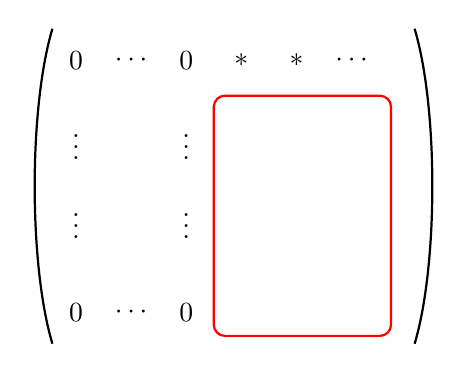
\begin{tikzpicture}[scale=1]
% outer matrix brackets
\draw[thick] (-0.3,0) .. controls (-0.6,1) and (-0.6,3) .. (-0.3,4);
\draw[thick] (4.3,0) .. controls (4.6,1) and (4.6,3) .. (4.3,4);

% first row: zeros before pivot, then entries after (pivot + rest)
\node at (0,3.6) {$0$};
\node at (0.7,3.6) {$\cdots$};
\node at (1.4,3.6) {$0$};
\node at (2.1,3.6) {$*$};
\node at (2.8,3.6) {$*$};
\node at (3.5,3.6) {$\cdots$};

% remaining rows: dots under the leading-zero columns (unreduced),
% and the submatrix (red box) covering columns after the pivot
\node at (0,2.6) {$\vdots$};
\node at (1.4,2.6) {$\vdots$};

\node at (0,1.6) {$\vdots$};
\node at (1.4,1.6) {$\vdots$};

\node at (0,0.4) {$0$};
\node at (0.7,0.4) {$\cdots$};
\node at (1.4,0.4) {$0$};

% red box: submatrix from pivot+1 column to last column, rows 2 to last
\draw[thick, red, rounded corners] (1.75,0.1) rectangle (4.0,3.15);
\end{tikzpicture}
\end{center}
\end{marginfigure}

Now, let us formally prove this.

\begin{proof}
We induct on the number of the rows. For a one-row matrix, if all the columns are zero
then the statement vacuously holds. Otherwise, let the pivot be $c \neq 0$. Scaling
by $1/c$ reduces it to the desired form.

Suppose we have shown this for matrices of number of rows $1, 2, \dots, k$. Consider a
matrix with $k+1$ rows. Find the first column with a non-zero element (if this does not
exist, the matrix is just the zero-matrix, so our statement is vacuously true). Swap the row containing this
to the top. Now, scale it by $1/c$ where $c$ is the value of the pivot. Consider now the rows
below the first row. Suppose they've entries $a_i$ is the pivot column.
Then, subtract $a_i$ times the first row from the $i$-th row, so that all of the
entries in the pivot column are now zero except the first row. Note that, now we can
just reduce a matrix of a smaller size (the submatrix formed by rows 2 through $k+1$) of
$k$ rows to a row-echelon form.

Since we do this using elementary row operations, which only involve
linear combinations and swapping, the columns containing $0$ can not be changed, as
swapping only changes $0$ to another $0$, and a linear combination of $0$ entries is also $0$. Therefore,
reducing it to a row-echelon form makes the whole matrix in a row-echelon form now
(as the next pivot is at least one column after the first pivot,
because all columns in the submatrix have zero entries up until the pivot column,
so the first pivot can only occur later (or never)).
\end{proof}

\begin{remark}
One may consider augmented matrices ad-hoc representations for now,
but there is a somewhat nice reason for considering them. These elementary
row operations correspond to multiplication by a specific kind of invertible matrix
(called an elementary matrix) i.e
\[
EA\mathbf{x} = E\mathbf{b} \iff A\mathbf{x} = \mathbf{b}.
\]

We will discuss them later, but in particular a property that our augmented matrix exhibits is:
\[
E(A \mid \mathbf{b}) = (EA \mid E\mathbf{b}).
\]

We can now look at \Cref{exm:equivalent-systems} in this manner.
Let us show how the row operations correspond to matrix multiplication.


\[
E = E_4 E_3 E_2 E_1 = \begin{pmatrix} 0 & 1/3 \\ 1/4 & -1/6 \end{pmatrix}, \qquad \det E = -\frac{1}{12} \neq 0
\]

\[
A = \begin{pmatrix} 2 & 4 & 6 & 8 \\ 3 & 0 & 7 & 1 \end{pmatrix}, \qquad \vec{b} = \begin{pmatrix} 1 \\ 10 \end{pmatrix}
\]

\[
EA = \begin{pmatrix} 0 & 1/3 \\ 1/4 & -1/6 \end{pmatrix} \begin{pmatrix} 2 & 4 & 6 & 8 \\ 3 & 0 & 7 & 1 \end{pmatrix} = \begin{pmatrix} 1 & 0 & 7/3 & 1/3 \\ 0 & 1 & 1/3 & 11/6 \end{pmatrix}
\]

\[
E\vec{b} = \begin{pmatrix} 0 & 1/3 \\ 1/4 & -1/6 \end{pmatrix} \begin{pmatrix} 1 \\ 10 \end{pmatrix} = \begin{pmatrix} 10/3 \\ -17/12 \end{pmatrix}
\]

\[
E(A \mid \vec{b}) = \begin{pmatrix} 0 & 1/3 \\ 1/4 & -1/6 \end{pmatrix} \left( \begin{array}{cccc|c} 2 & 4 & 6 & 8 & 1 \\ 3 & 0 & 7 & 1 & 10 \end{array} \right) = \left( \begin{array}{cccc|c} 1 & 0 & 7/3 & 1/3 & 10/3 \\ 0 & 1 & 1/3 & 11/6 & -17/12 \end{array} \right)
\]

\hrule

Thus may think of augmented matrices as \emph{representations}, or really, as the system of equations themselves,
and then the way of writing it down as the $r \times (c+1)$ table of numbers as a
\emph{representation}. One understands this as:

\end{remark}

\begin{question}
If the system is inconsistent, will the row-echelon form of the augmented matrix have rows of the form:
\[
\left(
\begin{array}{cccc|c}
0 & 0 & \cdots & 0 & c
\end{array}
\right)
\]
where $c \neq 0$.

\vspace{1em}
\hrule
\vspace{1em}

Yes, otherwise since we can reduce any augmented matrix to a row-echelon form,
and this swapping back of variables will lead us to a set of solutions.
\end{question}
